
The global \MPAS model uses Centroidal Voronoi Tesselation (CVT) to generate a variable resolution mesh that provides a smooth coastal to deep-ocean transition region and minimizes diffusive effects during long term termporal integration. However, the regional \ROMS model with typically a higher spatiotemporal resolution uses a curvilinear grid in the radial direction, leading to a regionally structured mesh embedded in an unstructured global polygonal mesh. We will discuss the problem setup, the complication due to variation in axial coordinate systems~\citep{petersen2015evaluation}, and describe the algorithm that achieves consistent embeddings to transfer the forcing conditions accurately and efficiently.

\subsection{Problem statement and notation}\label{sec:problem}

The central design constraint is that the source and target
discretizations differ in \emph{both} the horizontal tessellation
(unstructured Voronoi vs.\ structured curvilinear) \emph{and} the
vertical coordinate (fixed-$z$ vs.\ terrain-following sigma), as
illustrated in Figure~\ref{conv:fig:coord-mismatch}. 


Let the {\MPAS} global ocean mesh cover a region of interest with
$n_M$ Voronoi cells, each carrying a column of tracer values on
$K_M$ fixed depth levels $\{\zmpas_k\}_{k=1}^{K_M}$. Let the \ROMS{}
target grid have $n_R$ horizontal cells, each with a column of
$K_R$ terrain-following (sigma) levels whose absolute depths
$\{\zmpas_\ell^{(i)}\}_{\ell=1}^{K_R}$ depend on the local bathymetry
$H_i$ and free-surface elevation $\zeta_i$ through the Song--Haidvogel
stretching transformation~\citep{song1994semi,shchepetkin2005regional}.
A three-dimensional \MPAS source field is then given by the array
$\Phi \in \mathbb{R}^{n_M \times K_M}$ and the projected \ROMS 
regional target field is $\Psi \in \mathbb{R}^{n_R \times K_R}$. The problem at hand is to compute consistent, and conservative three-dimensional solution transfer from global \MPAS models to the \ROMS model to achieve one-way submesoscale resolving solutions.

Note that a fully
three-dimensional intersection of two such cell complexes is possible, but in general will involve $O(n_M n_R K_M K_R)$ computational complexity to decipher candidate overlaps (worst case),
and can produce multiple sliver polyhedra whose quadratures are ill-conditioned.
We instead exploit the fact that the \MPAS{} vertical coordinate is
horizontally uniform (the depth levels $\zmpas_k$ do not vary between
columns) to factor the transfer into a horizontal remap and a
one-dimensional vertical remap.


\begin{figure}[htbp]
\centering
\begin{subfigure}{0.43\textwidth}
	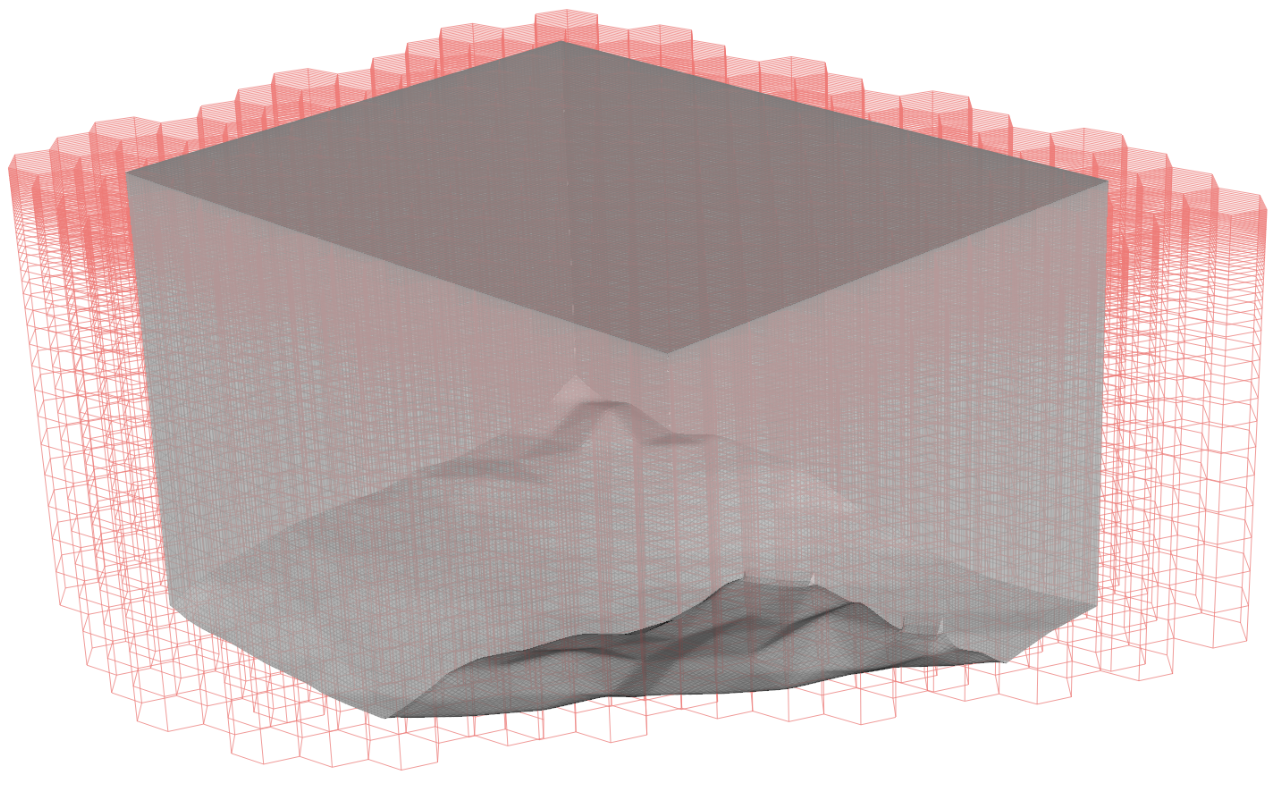
\includegraphics[width=\textwidth]{Figures/conv_embedded_3dmesh.png}
	\caption{Regional \ROMS mesh embedded within the \MPAS source domain.}
	\label{conv:fig:embed3d}
\end{subfigure}\hfill
\begin{subfigure}{0.55\textwidth}
	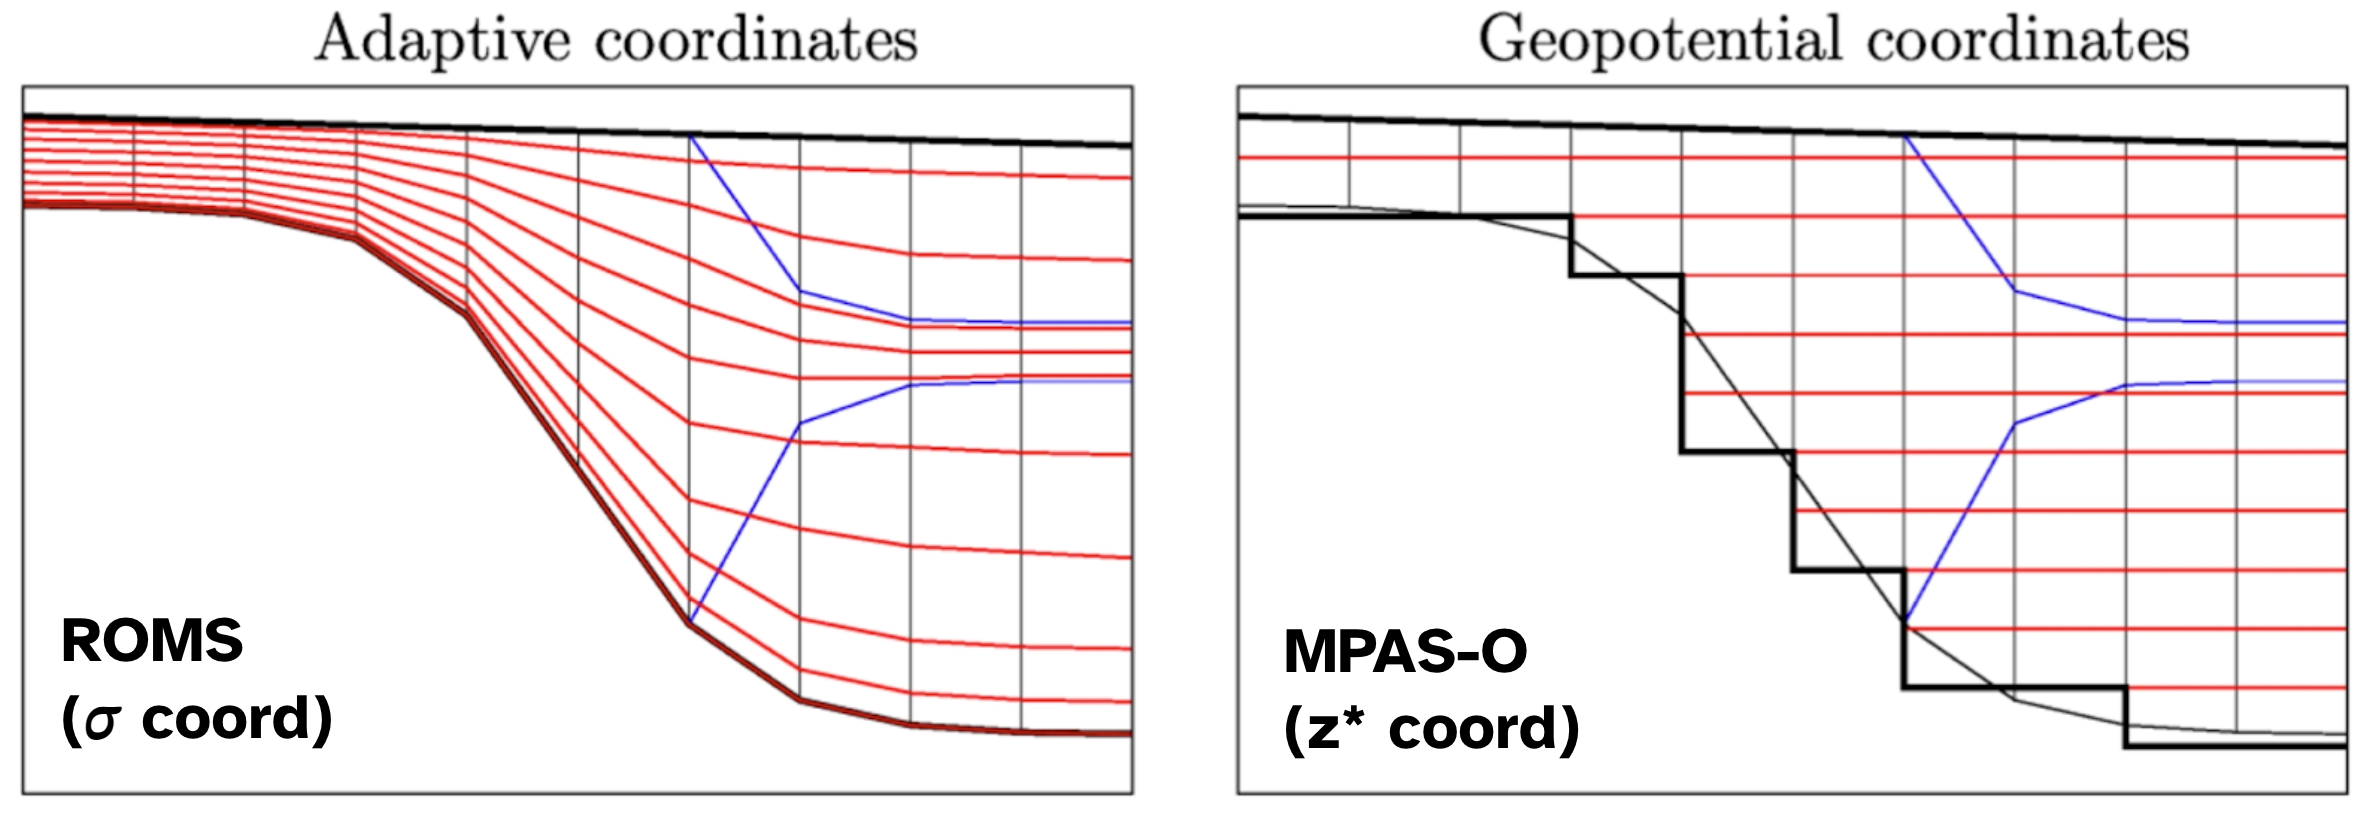
\includegraphics[width=\textwidth]{Figures/conv_zcoord_contrast.png}
	\caption{\ROMS terrain following ($\sigma$) and \MPAS geopotential ($z^*$) coordinates.}
	\label{conv:fig:zcoord}
\end{subfigure}
\caption{Horizontal (left) and vertical (right) discretizations used in the transfer.}
\label{conv:fig:coord-mismatch}
\end{figure}

Throughout the manuscript, we indicate source \MPAS cell indices with the subscript $j$, and target \ROMS cells with the $i$ index, while $k$ and $\ell$ index source and target vertical levels respectively. Uppercase $\Phi,\Xi,\Psi$ denote whole
three-dimensional arrays, and the corresponding lowercase $\phi,\psi$
denote a single horizontal slab extracted at a fixed level, so that
$\phi_j=\Phi_{j,k}$ for the level $k$ under discussion. Cell areas carry the mesh as a superscript: $A^M_j$ is the
area of source cell $j$, $A^R_i$ that of target cell $i$, and $A_{ij}$
the area of their intersection. All geometry is treated on the unit
sphere, areas are spherical areas computed by L'Huilier's excess
formula, and horizontal weights are area-based so that the operators
are independent of the absolute mesh radius.

% Methods section.
\subsection{Separable volumetric remapping}\label{conv:sec:methods}

Writing $\Xi$ for the intermediate field that results from transferring
every source level horizontally, and $\mathcal{V}$ for the column-wise
vertical remap, the composed transfer is
\begin{equation}
  \Xi_{i,k}=\sum_j W_{ij}\Phi_{j,k},\qquad \Psi=\mathcal{V}(\Xi),
  \label{conv:eq:tensor}
\end{equation}

where the horizontal map $W$ is reused unchanged at every source level
and $\mathcal{V}$ acts independently on each target column. This
prism-based 2D$\times$1D construction avoids sliver polyhedra while
retaining the column geometry that the vertical remap requires. The two
factors are developed in turn in \S\ref{sec:horizontal} and
\S\ref{sec:vertical}. A schematic of the volumetric remapping algorithm is shown in Figure~\ref{fig:remap_methods}.


\begin{figure}[htbp]
	\centering
	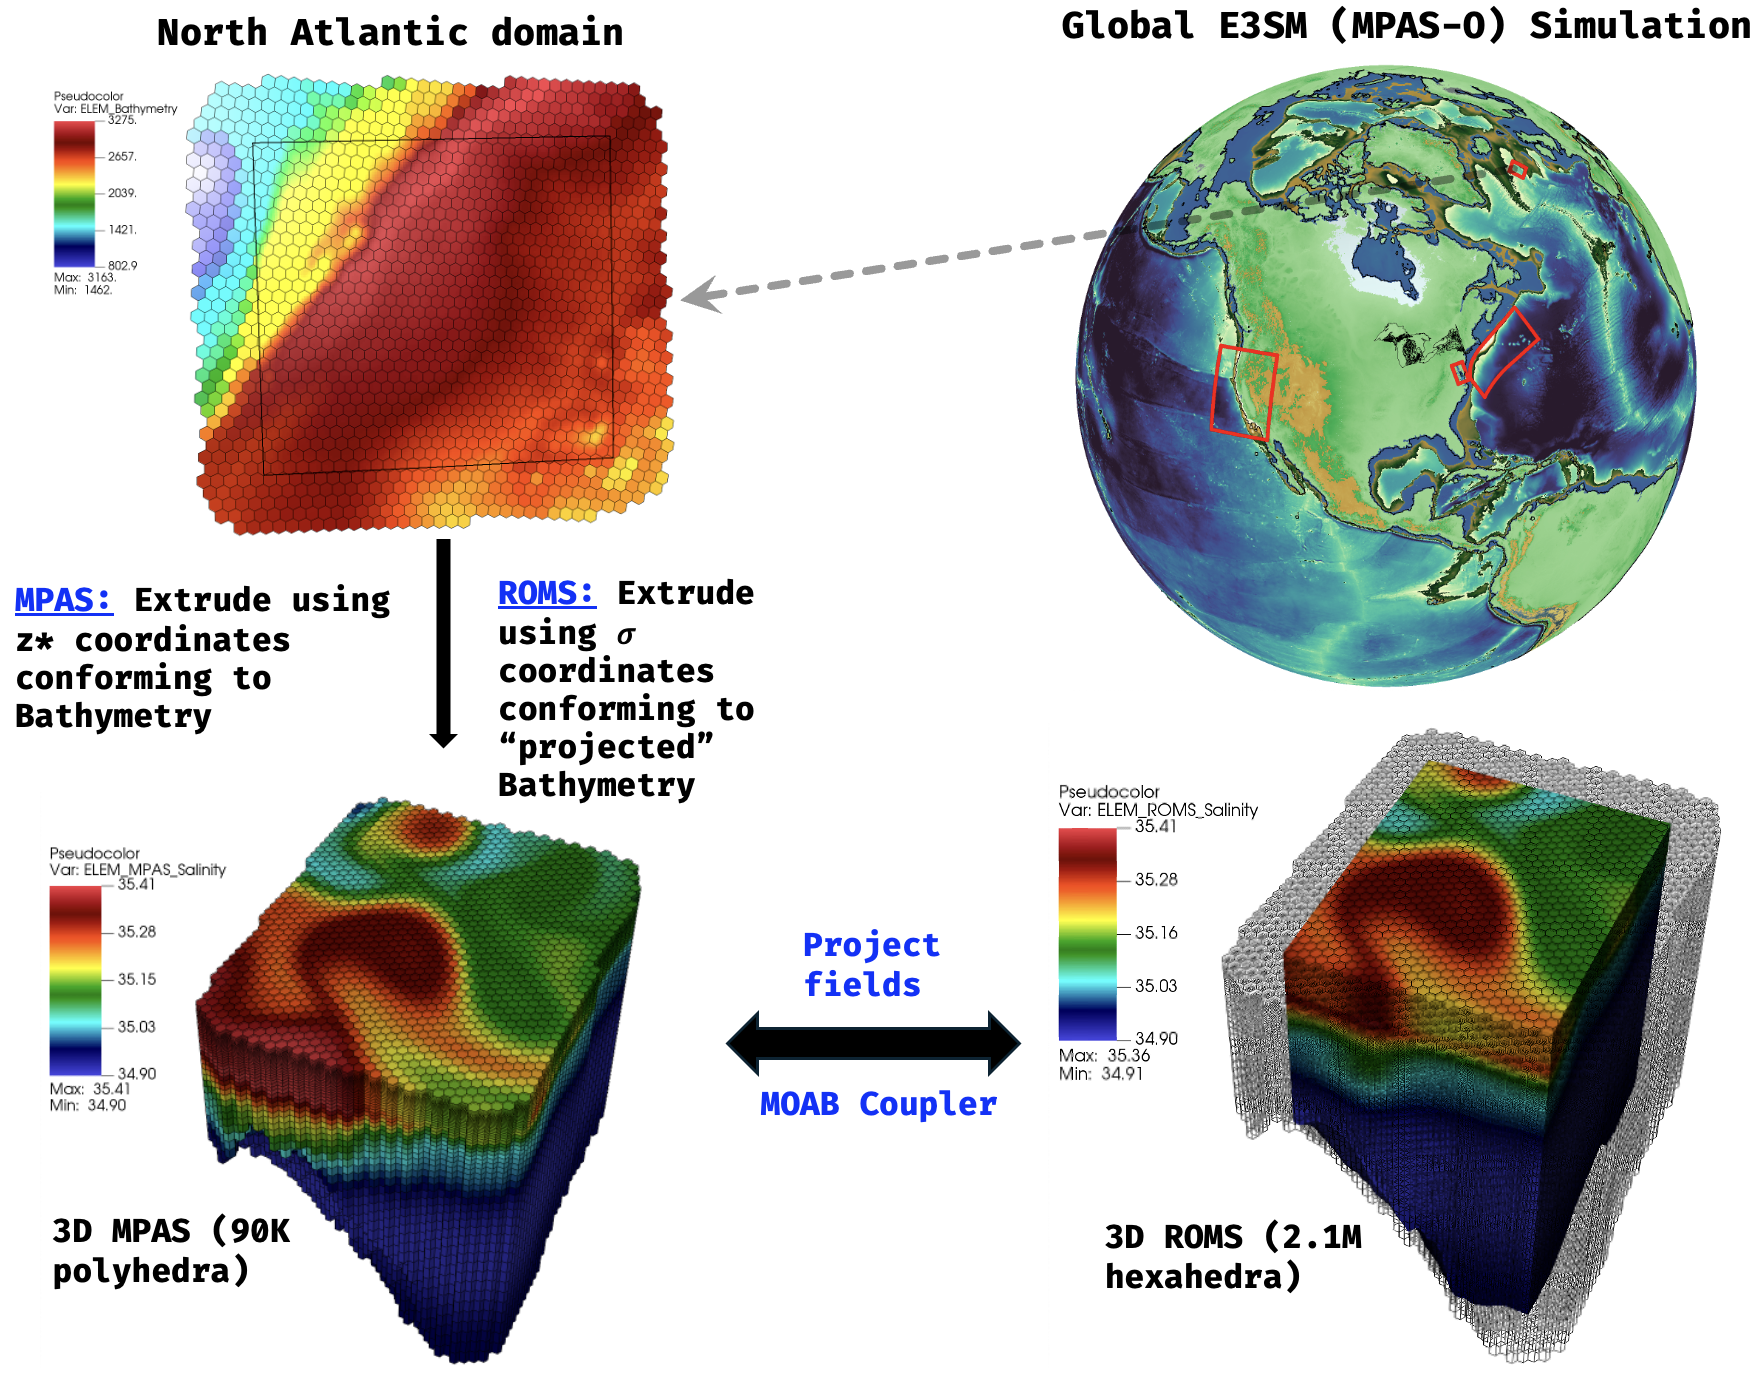
\includegraphics[width=\textwidth]{Figures/remapping_schematics.png}
	\caption{Schematic of the offline volumetric transfer and regional domains.}
	\label{fig:remap_methods}
\end{figure}


\subsection{Horizontal remap as a sparse linear map}\label{sec:horizontal}

There are different remapping choices that one could utilize to take the 2D surface layer from \MPAS and project it to an embedded \ROMS regional domain. The standard approach is to use the $L_2$ minimization that preserves both the global and local integrals of the fields for exact conservation. However, due to the disparity in the resolution between the \MPAS and \ROMS meshes, the coarse-to-fine projections can yield severe mesh imprinting artifacts as demonstrated by experiments on the North-Atlantic domain in Fig.~\ref{fig:mesh-imprinting}. Here, the \MPAS meshes are about \emph{5x} coarser than the \ROMS meshes, which is already yielding severe imprinting, which can cause instability in the \ROMS simulations.

For a fixed source depth level $k$, the horizontal factor $W$ of
Eq.~\eqref{conv:eq:tensor} acts on the level slab
$\phi=\Phi_{:,k} \in \mathbb{R}^{n_M}$ as the sparse linear map
\begin{equation}
	\psi_i \;=\; \sum_{j=1}^{n_M} W_{ij}\, \phi_j ,
	\qquad W \in \mathbb{R}^{n_R \times n_M},
	\label{eq:linear-map}
\end{equation}
in the linear-maps-for-remapping sense
of~\citet{ullrich2015arbitrary,ullrich2016tempestremap}. Two
constructions of the weights in Eq.~\eqref{eq:linear-map} are
considered below, and they differ in whether conservation or
smoothness is enforced.

\paragraph{Conservative finite-volume (FV) map.}
The first-order conservative finite-volume linear-map ~\citep{jones1999scrip} is computed based on the full supermesh in order to account for the contributions from all partial subcell geometry neighbors from the source mesh overlapping the target elements. This sets the
weight to the area of geometric overlap between target cell $i$ and
source cell $j$, normalized by the target area,
\begin{equation}
	W^{\mathrm{FV}}_{ij} \;=\; \frac{|\Omega_i \cap \Omega_j|}{|\Omega_i|}
	\;=\; \frac{A_{ij}}{A^R_i},
	\label{eq:fv-weight}
\end{equation}
where $\Omega_i$, $\Omega_j$ are the (spherical) target and source
polygons and $A_{ij}$ their intersection area. This map is
\emph{conservative only over the target-covered subdomain}, a
qualification that matters here because the \ROMS{} target is a bounded
region embedded in a global \MPAS{} source: because
$\sum_i A_{ij} = A^M_j$ holds only for a source cell fully covered by the
union of target cells, the area-weighted integral identity
$\sum_i A^R_i \psi_i = \sum_j A^M_j \phi_j$ is exact for source cells
interior to the target footprint and is broken for source cells that
the limited-domain target only partially overlaps. Conservation
therefore applies to the covered interior, never to the source cells
straddling the target boundary; this is the boundary qualification we
enforce operationally through the interior/partial classification of
\S\ref{sec:classification}. The map is first-order accurate and, being
a convex average of the source values ($W^{\mathrm{FV}}_{ij}\ge 0$,
$\sum_j W^{\mathrm{FV}}_{ij}=1$ on fully-covered cells), it is
unconditionally monotone.

\paragraph{Normalized bilinear map.}
The bilinear map locates each target-cell centroid within the source
\MPAS triangulation, forms bilinear interpolation weights
$b_{ij}$ from the enclosing source elements, and row-normalizes them, following the linear-map framework of~\citet{ullrich2015arbitrary,ullrich2016tempestremap}.
\begin{equation}
	W^{\mathrm{BL}}_{ij}
	\;=\; \frac{b_{ij}}{\sum_{j'} b_{ij'}} ,
	\label{conv:eq:bilin-weight}
\end{equation}
so that constant fields are reproduced exactly
($\sum_j W^{\mathrm{BL}}_{ij}=1$). The bilinear map is not globally
conservative by construction, since its column sums are not area ratios Equation.~\ref{eq:fv-weight}. It is, however, second-order accurate on smooth fields and, more importantly for the downscaling setup, it does not tie the target values to the piecewise-constant average of a single source cell. The nonnegative weights form a convex combination that preserves the range of contributing source values, so the map is property-preserving. Its second-order horizontal accuracy does not raise the order of the composed transfer, which is limited by the conservative vertical remap of \S\ref{sec:vertical}, as discussed in \S\ref{conv:sec:conv}.



\subsection{Issues with conservative FV map for tracers}\label{sec:why-not-fv}

The conservative finite-volume (FV) map in \eqref{eq:fv-weight} is the lowest-order case of the conservative \(L_2\)-minimization framework used for general mesh remapping \citep{ullrich2015arbitrary,ullrich2016tempestremap}. Given compatible source and target bases, the transferred field minimizes the overlap-domain error
\begin{equation}
	\int_{\Omega}(f-g)^2\,\mathrm{d}\Omega ,
	\label{eq:l2-min}
\end{equation}
leading to a discrete system $W_{S\rightarrow T}G=F$. Higher-order conservative, monotone, and smooth alternatives are available \citep{lauritzen2008monotone,lee1997mba}; here we focus on the first-order FV map and the normalized bilinear map in \eqref{conv:eq:bilin-weight}, which capture the main trade-off relevant to MPAS--ROMS downscaling.

We retain the FV map for coverage classification (\S\ref{sec:classification}), since its overlap-area weights provide a meaningful geometric coverage fraction. We do not use it for tracer transfer, however, because it produces mesh imprinting.

In the configurations considered here the \ROMS cells are typically much smaller than the \MPAS ocean model cells, that is $\hRatio\ll1$. Under first-order FV remapping, all fine target cells lying within a given \MPAS Voronoi cell receive the same source-cell average. The resulting field is therefore piecewise constant on the source tessellation, even though it is represented on the fine ROMS grid. This appears as a staircase pattern whose discontinuities follow MPAS cell edges.

These discontinuities are not physical gradients. They are introduced solely by the transfer operator and can inject grid-scale noise or adjustment features aligned with the source mesh when the field is used to initialize or force a regional model. The problem is especially consequential for fields that should vary smoothly at the regional scale.

The normalized bilinear map removes the leading-order imprint by interpolating continuously across source mesh rather than assigning constant cell averages, at the cost of exact global conservation. For boundary and initial-condition forcing we regard this as an acceptable compromise, since \ROMS evolves its tracer inventory with its own conservative transport scheme, whereas mesh-imprinted forcing introduces artificial gradients that can persist in the interior solution. The argument does not extend to applications that require strict conservation of the horizontally transferred inventory; those would need an additional correction.

The verification metrics reported here, $\Lone$, $\Ltwo$, and $\Linf$ of Eq.~\eqref{conv:eq:norms}, assess pointwise round-trip accuracy rather than the global horizontal inventory error
\begin{equation}
	\left|\sum_i A^R_i\psi_i-\sum_j A^M_j\phi_j\right| .
	\label{eq:inventory-error}
\end{equation}
Vertical conservation, where needed, is provided separately by the operator of \S\ref{sec:vertical} without reintroducing horizontal imprinting.

Figure~\ref{fig:mesh-imprinting} demonstrates the effect using projected bathymetry over the refined North Atlantic domain. The FV result (centre) reproduces the MPAS Voronoi tessellation as piecewise-constant patches with sharp artificial steps, while the normalized bilinear result (right) remains smooth. Bathymetry provides a useful example because it directly affects the ROMS sigma-coordinate geometry; imprinting in the transferred field therefore perturbs the vertical grid as well as the horizontal representation.


\begin{figure}[htbp]
	\centering
	\begin{subfigure}{0.29\textwidth}
		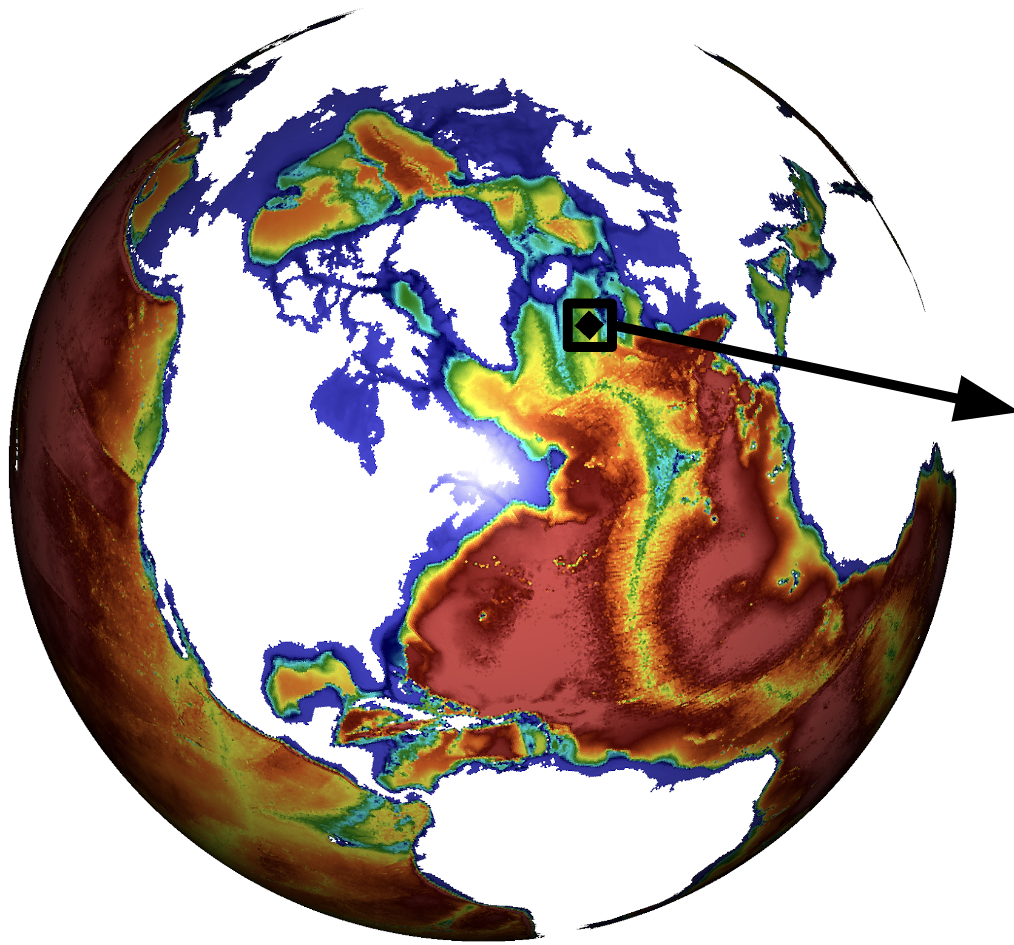
\includegraphics[width=\textwidth]{Figures/fig_regional_refinement.png}
		\caption{Regionally refined domain.}
		\label{fig:imprint-region}
	\end{subfigure}\hfill
	\begin{subfigure}{0.35\textwidth}
		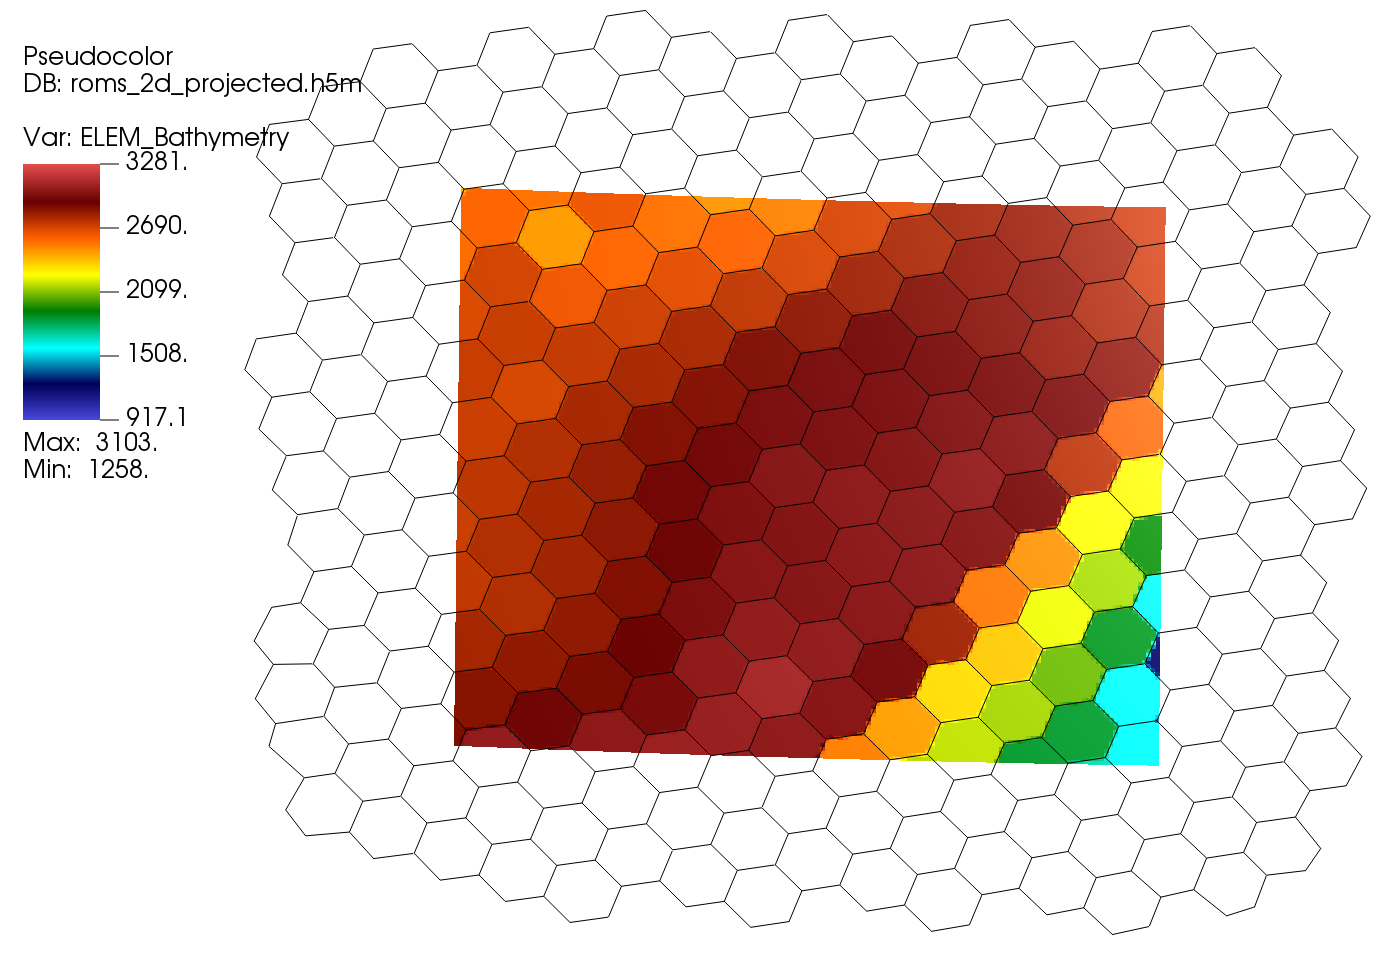
\includegraphics[width=\textwidth]{Figures/conv_bathy_fv.png}
		\caption{Conservative FV ($L_2$-minimizing) map.}
		\label{conv:fig:fv-remap}
	\end{subfigure}\hfill
	\begin{subfigure}{0.35\textwidth}
		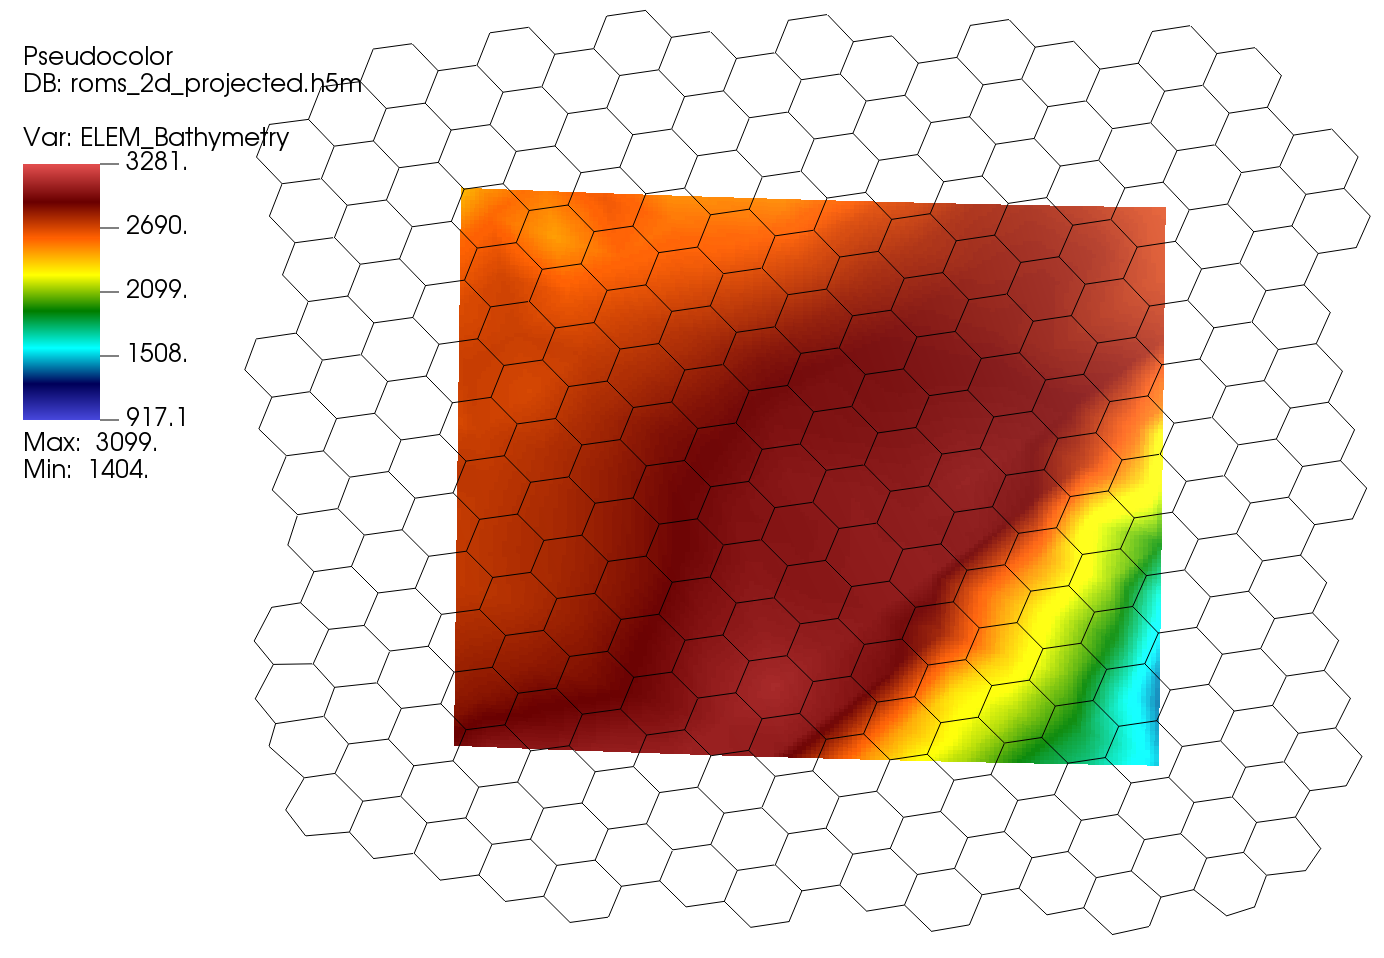
\includegraphics[width=\textwidth]{Figures/conv_bathy_bilinear.png}
		\caption{Bilinear projection.}
		\label{conv:fig:bilinear-remap}
	\end{subfigure}
	\caption{Mesh imprinting in the North Atlantic domain. The conservative FV map reproduces the \MPAS Voronoi tessellation as piecewise-constant patches, whereas the normalized bilinear map remains smooth.}
	\label{fig:mesh-imprinting}
\end{figure}


\subsection{Vertical remap of each column}\label{sec:vertical}

Each intermediate column is assigned physical source depths taken from the nearest source column, and is then remapped onto the local target depths using a monotone, piecewise cubic-Hermite interpolant (PCHIP), where the terrain-following depths follow from the target bathymetry and free-surface ocean elevation (SSH). The property preserved in the vertical direction is the integral of the reconstructed point-sampled profile over each target layer, which for piecewise average degrees-of-freedom originating from finite-volume solvers results in a remap of source-layer averages. Outside the source depth range the profile is held at the nearest endpoint rather than extrapolated for tracer fields, and velocities are maintained at zero.


The linear map is assembled separately for each direction and is independent of level and field. It is important to note that to supply a full level slab, values below the deepest wet source level (\MPAS axial layer masking) are held at the deepest wet value, resembling nearest neighbor extrapolation. The extended tail is discarded when the column is restricted to its physical depth range. This is held true for true tracers, while velocity fields are zeroed out during extrapolation (no flow conditions). The implications of these approaches to handling strong bathymetry variations will be discussed later.


%We should emphasize that these are properties of the two component operators. Neither individually, nor in combination, do they guarantee that the composed three-dimensional transfer conserves volume-integrated quantities or preserves bounds.

It is noted that the zonal and meridional velocities are transferred component-wise as scalar, Earth-relative fields at horizontal cell centers. No rotation to the curvilinear basis, interpolation to polygonal edges, or discrete divergence constraints are imposed in this transfer. The velocity diagnostics presented in this manuscript measure componentwise transport in a fixed basis. Use of consistent mimetic schemes to dynamically transfer vector fields remains outside the present scope of the paper and will be pursued in future work.

\subsection{Regional domains and metrics}\label{conv:sec:regional-methods}


\TODOc{Kyle: Need to add more details about the metrics that we care about in regional domains. Provide details about nudging, and how \ROMS utilizes the time-dependnet forcing conditions to get a consistent view of the global solution}


The solution verification uses the Gulf Stream and Bay of Bengal domains, while regional application validation also include the North Atlantic and Chesapeake Bay. Regional interpretation relies on relative-vorticity maps and surface kinetic-energy time series.
